\documentclass[10pt,a4paper]{article}
\usepackage[english]{babel}
\usepackage[utf8]{inputenc}
\usepackage{amsmath}
\usepackage{amsfonts}
\usepackage{amssymb}
\usepackage{graphicx}
\usepackage{float}
\usepackage{caption}

%link to documentation: 
%https://ackrep-doc.readthedocs.io/en/latest/devdoc/contributing_data.html

\begin{document}
	\part*{Model Documentation of the \\ Ball and Beam} % MUST - Add Model Name 
	
	%%%%%%%%%%%%%%%%%%%%%% NOMENCLATURE %%%%%%%%%%%%%%%%%%%%%%%%%%%
	
	\section{Nomenclature} % MUST
	\subsection{Nomenclature for Model Equations} % MUST
	
	%variables for model equations
	\begin{tabular}{ll}
		$m_1$ & mass of the ball \\
		$J_1$ & moment of inertia of the beam \\
		$J_2$ & moment of inertia of the ball \\
		$r$ & radius of the ball \\
		$g$ & acceleration due to gravity \\
		$\tau$ & torque in the middle of the beam \\
		$q_1$ & distance between the ball and the middle of the beam \\
		$q_2$ & rotation angle of the beam \\
				
	\end{tabular}
	 
	\subsection{Graphic of the Structure}	
	\begin{figure}[H]
		\centering
		\captionsetup{justification=centering, margin=1cm}
		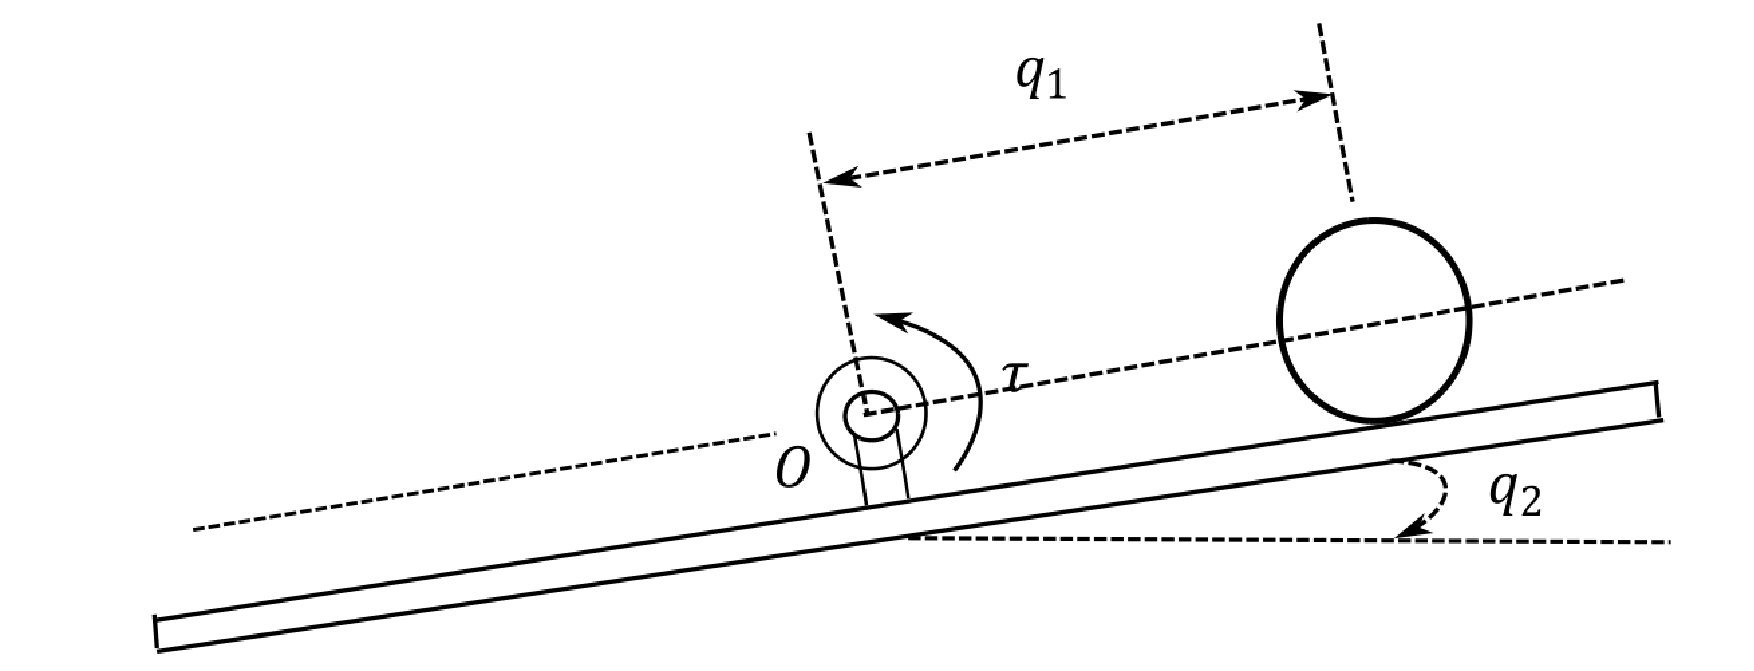
\includegraphics[width=70mm]{ball_beam.pdf}
		\caption{Structure of the Ball and Beam \\ \footnotesize{Source: Wang, Yang/Erstellung eines regelungstheoretischen Katalogs unteraktuierter mechanischer Systeme}}
	\end{figure}
	
	%%%%%%%%%%%%%%%%%%%%%% MDOEL EQUATIONS %%%%%%%%%%%%%%%%%%%%%%%%%%%
	
	\section{Model Equations} % MUST
	
	State Vector and Input Vector:
	\begin{align*}
		\underline{x} &= (q_1 \ q_2 \ \dot{q}_1 \ \dot{q}_2)^T &= (x_1 \ x_2 \ x_3 \ x_4)^T\\
		\underline{u} &= \tau &= u_1  
	\end{align*}
	
	\noindent System Equations:			
	\begin{subequations}
	\begin{align}
		\dot{x}_1 &= x_3 \\
		\dot{x}_2 &= x_4 \\
		\dot{x}_3 &= \frac{m_1x_1x_4^2 - gm_1\sin x_2}{m_1 + \frac{J_2}{r^2}}\\
		\dot{x}_4 &= \frac{\tau - m_1gx_1 \cos x_2 - 2m_1x_1x_3x_4}{J_1 + J_2 + m_1x_1^2}		
	\end{align}
	\end{subequations}

	%%%%%%%%%%%%%%%%%%%%%% PARAMETERS | OUTPUTS %%%%%%%%%%%%%%%%%%%%%%%%%%%
	\noindent
	Parameters:  $m_1, \, J_1 , \, J_2, \, r, \, g$ % variables with constant, predefined value
	\\
	Outputs: $\underline{x}$ 
	
	
	%%%%%%%%%%%%%%%%%%%%%% EXEMPLARY PARAMETER VALUES %%%%%%%%%%%%%%%%%%%%%%%%%%%	
	
	\subsection{Exemplary parameter values}
	\begin{tabular}{cl}
\hline
  Symbol  & Value                                                                                                                                                                                \\
\hline
   $A$    & $\left[\begin{matrix}0.8189 & 0.0863 & 0.09 & 0.0813\\0.2524 & 1.0033 & 0.0313 & 0.2004\\-0.0545 & 0.0102 & 0.7901 & -0.258\\-0.1918 & -0.1034 & 0.1602 & 0.8604\end{matrix}\right]$ \\
   $B$    & $\left[\begin{matrix}0.0045 & 0.0044\\0.1001 & 0.01\\0.0003 & -0.0136\\-0.0051 & 0.0936\end{matrix}\right]$                                                                          \\
 $B_{1}$  & $\left[\begin{matrix}0.0045 & 0.0044\\0.1001 & 0.01\\0.0003 & -0.0136\\-0.0051 & 0.0936\end{matrix}\right]$                                                                          \\
 $C_{1}$  & $\left[\begin{matrix}1.0 & 0 & -1.0 & 0\\0 & 0 & 0 & 0\\0 & 0 & 0 & 0\end{matrix}\right]$                                                                                            \\
   $C$    & $\left[\begin{matrix}1.0 & 0 & 0 & 0\\0 & 0 & 1.0 & 0\end{matrix}\right]$                                                                                                            \\
 $D_{11}$ & $\left[\begin{matrix}0 & 0 & 0\\0 & 0 & 0\\0 & 0 & 0\end{matrix}\right]$                                                                                                             \\
 $D_{12}$ & $\left[\begin{matrix}0 & 0\\1.0 & 0\\0 & 1.0\end{matrix}\right]$                                                                                                                     \\
 $D_{21}$ & $\left[\begin{matrix}0 & 1.0 & 0\\0 & 0 & 1.0\end{matrix}\right]$                                                                                                                    \\
\hline
\end{tabular}

	%%%%%%%%%%%%%%%%%%%%%% DERIVATION & EXPLANATION %%%%%%%%%%%%%%%%%%%%%%%%%%%	
	
	\section{Derivation and Explanation} % SHOULD
	The Lagrangian mechanics was used for the solution. \\
	Rotational Energy: 
	\begin{align}
		T_{rball} &= \frac{1}{2}J_2x_4^2 + \frac{1}{2} \frac{J_2}{r^2} x_3^2 \\
		T_{rbeam} &= \frac{1}{2}J_1x_4^2
	\end{align}
	Translational Energy: 
	\begin{align}
		T_{t} = \frac{1}{2}m_1(x_3^2 + x_1^2x_4^2)
	\end{align}
	Potential Energy: 
	\begin{align}
		V = m_1gx_1 \sin x_2
	\end{align}
	
	%%%%%%%%%%%%%%%%%%%%%% REFERENCES %%%%%%%%%%%%%%%%%%%%%%%%%%%
	
	\begin{thebibliography}{10}		
		\bibitem{But21}Wang, Yang: 
		\textit{Erstellung eines regelungstheoretischen Katalogs unteraktuierter mechanischer Systeme}, master thesis at the Institut of Control Theory TU Dresden, published 2016. \\
		(not publicly accessible)
	\end{thebibliography}

\end{document}

